% !Mode:: "TeX:UTF-8"%確保文檔utf-8編碼
%新加入的命令如下: reduline showendnotes 
%新加入的环境如下:solution solutionorbox solutionorlines solutionordottedlines

\documentclass[12pt]{exam}
\newlength{\textpt}
\setlength{\textpt}{12pt}

\usepackage{teachingplan}
\usepackage{parallel}
%输出方案 
%学生版 学霸版 老师版

%写上答案或者不写上答案%1  
\printanswers  

%提高题
%\includecomment{advanceexercises}
\excludecomment{advanceexercises}


\CenterWallPaper{1}{教案模板-2.pdf}

\newcommand{\keti}{物质的微观视角}
\newcommand{\zhongdian}{1.物质是由分子组成的  2.温度 3.物态变化  4.理解压强 5.理解化学反应   }

\begin{document}
\ThisCenterWallPaper{1}{教案模板-1.pdf}
\vspace*{80pt}
\keti \par
\zhongdian \par
\section{物质是由分子组成的}
播放视频:从夸克到宇宙

我们眼睛朝外望,获得的第一个观念就是这个世界充满了各种各样的物质,比如说这根粉笔,再比如说桌子椅子。

这些物质都有什么性质啊?是的他们都具有质量而且还占据了一定的空间。

首先我们的第一个问题是:物质都是由什么构成的呢?

在遥远的古希腊有一个人名叫徳谟克利特,他相信世界上所有的物质都是由原子构成的。不过他所谓的原子估计是看到岩石变成沙子,沙堆里分沙子的模型构想出来的,他的原子的概念简单来说就是一种无比坚硬的东西,因为它无比坚硬所以没有什么刀(或者其他作用)能把它分开了,这就是他所谓的原子。而现代的原子概念和他说的原子概念区别还是很大的。

那么如果我们把沙子一直分下去,最后会得到什么?沙子主要是由一种叫\chemfig{SiO_2}的分子组成的,而一个二氧化硅分子又是由一个硅原子和两个氧原子构成的。原子由内部小小的原子核和外面到处乱跑的电子构成的。原子核是由质子和中子构成的(氢原子核里面只有质子没有中子)。质子和中子又是由夸克构成的。那么夸克是物质的最小的构成单位吗?

同时我们在思考物质的微观构造的时候还有一种思路,我们关心的是物质的性质,而不是最小的构成单位。比如在古希腊还有一种说法认为物质是由水、火、气、土四种元素组成的。因为我们从水中看到了流动性,从火中看到了热,从气中看到了飘忽不定,从土中看到了固体的特性。而在古代的中国也有一种类似的学说那就是五行学说,认为世界上的物质是由金木水火土四种元素组成的,而且古代中国人在分析问题的时候来引入了阴阳相生相克之理。

这一种思路发展到现代就构成了我们现代的分子概念,分子是保持物质化学性质的最小粒子。那么这是什么意思呢?意思就是如果你把盐的分子改变了盐就不是盐了,而对于盐你可以说就是盐分子组成的,对于木头你可以说就是木头分子组成的(假设木头不是混合物是一种纯净物。)

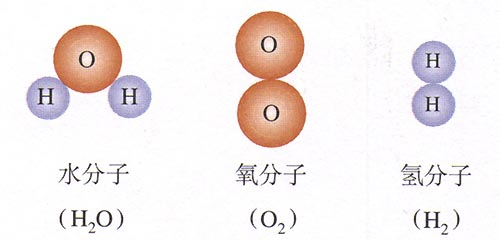
\includegraphics[width=\linewidth]{figures/氢分子氧分子和水分子.jpg} 

虽然我们不知道物质的最小构成单位是什么?但我们是可以说物质是由分子组成的。氧气是由氧气分子组成的,氢气是由氢气分子组成的,水是由水分子组成的。意思就是很多很多水分子聚集在了一起就组成了水。决定水之为水的就是水分子。


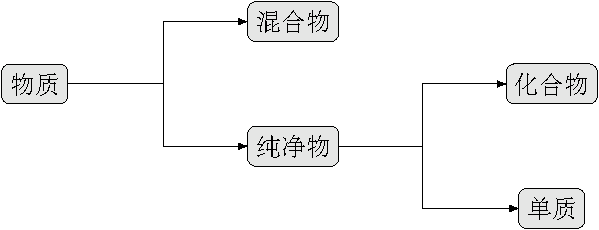
\includegraphics[scale=1]{figures/物质分类.pdf} 



\section{温度}
如果我们将水放大10亿倍,我们看到的水是什么样子呢?下面就物态变化和温度的关系具体说开去。
\begin{fig}{放大10亿倍的水}
\end{fig}


这是一张静态图片,实际上水分子在不停的运动着(还记得热和能一章我们学过一切物质的分子都在做无规则的运动,这种运动叫做热运动。)。这些分子热运动的剧烈程度在宏观上就反应了物质温度的大小。运动剧烈的分子会慢慢将能量传递给那些运动不剧烈的分子,这就是热量的传递。热量总是从温度高的地方传到温度低的地方。(热量总是自发的从温度高的地方传到低的地方,直到温度平衡。这正是接下来我们定义和测量温度的依据。)


定义:温度表示物体的冷热程度。

温度常用单位是摄氏度(℃) 规定:在一个标准大气压下冰水混合物的温度为$0$度,沸水的温度为$100$度,它们之间分成100等份,每一等份叫1摄氏度。某地气温$-3$℃读做:零下3摄氏度或负3摄氏度。


\subsection{温度计}
测量——温度计(常用液体温度计)

温度计的原理:利用液体的热胀冷缩进行工作。(其实还要加上一句热平衡状态下的两个物体温度相等。)

常用温度计的使用方法:
使用前:观察它的量程,判断是否适合待测物体的温度;并认清温度计的分度值,以便准确读数。使用时:温度计的玻璃泡全部浸入被测液体中,不要碰到容器底或容器壁;温度计玻璃泡浸入被测液体中稍候一会儿,待温度计的示数稳定后再读数;读数时玻璃泡要继续留在被测液体中,视线与温度计中液柱的上表面相平。


\section{汽化和液化}
物质从液态变为气态叫汽化。从气态变为液态叫做液化。就水的三态变化详细说明之。(如何运动?放热还是吸热?)

\begin{fig}{空气中水的蒸发}
\end{fig}

同样还有水蒸汽:
\begin{fig}{水蒸气}
\end{fig}


\subsection{沸腾}
在一定温度下,在液体内部和表面同时发生的剧烈的汽化现象。(沸腾现象和蒸发现象区别的核心点就是沸腾在液体内部也发生汽化,你能分析为什么吗?请联系液体内部压强和高压锅原理解释之。)

沸点:液体沸腾时的温度。(如果提高火炉的输出热量,请用汽化吸热和平衡来说明为什么液体存在沸点?如果提高火炉输出热量,将会有更多的具有更大动能的分子他们都将跑出液体,为什么液体的温度会保持不变。)

沸腾条件:(1)达到沸点。(2)继续吸热 

沸点与气压的关系:一切液体的沸点都是气压减小时降低,气压增大时升高。(外面气压大,液体分子就不容易跑出去。)


\subsection{蒸发}
液体在任何温度下都能发生的,并且只在液体表面发生的汽化现象叫蒸发。


影响因素:(1)液体的温度;(2)液体的表面积;(3)液体表面空气的流动。
\leftnote{如何影响}

作用:蒸发吸热(吸外界或自身的热量),具有制冷作用。生活中的热汤吹吹就凉了,主要是蒸发吸的热,你还能想出生活中其他应用吗?


例题:(2005年益阳)某年盛夏,在巴尔干地区,一农妇看见在野外考查有一位植物学家热得汗流浃背,便决定送杯牛奶给他喝。于是,农妇将盛牛奶的瓦罐用湿毛巾左一层右一层包严实后,放在太阳底下晒了一会儿,然后倒给植物学家喝,她这样做的目的是(\answerline*[A])
\begin{choices}
\choice 湿毛巾上的水在太阳光下曝晒迅速蒸发吸热,使牛奶温度降低
\choice 这是为了给牛奶加热
\choice 牛奶蒸发吸热,温度降低
\choice 这是利用太阳光杀菌
\end{choices}

\subsection{液化}
物质从气态变为液态叫液化。

方法:(1)降低温度;(2)压缩体积。好处:体积缩小便于运输。作用:液化放热

例题:(2007年北京)夏天打开冰箱时,在冰箱门附近会形成“白气”,形成“白气”的物态变化过程是(\answerline*[C])

\begin{oneparchoices}
\choice 升华
\choice 汽化
\choice 液化
\choice 熔化
\end{oneparchoices}

例题:(2005年桂林)夏天,从冰箱中取出瓶装矿泉水时,会发现瓶外壁“出汗”,这是(\answerline*[B])
\begin{choices}
\choice 水从瓶内渗出来的结果
\choice 空气中水蒸气遇冷的液化现象
\choice 空气中水蒸气的汽化现象
\choice 瓶外壁上的水汽化产生的现象
\end{choices}


\section{固体的讨论}
严格意义上讲任何物质在固态都会达到一种能量(就是大家各就各位坐在座位上挤得紧紧的也不到处乱跑)最低时候的状态,这个时候的固体就是\textbf{晶体}。只是有些物质在相当长的时间内都不能形成晶体,他们通常被称之为粘稠的液体或者凝固了的液体。比如塑料,橡胶,玻璃,蜡烛等。像这些物质(\textbf{非晶体})都没有确定的熔点。
\begin{fig}{食盐的晶体结构}
\end{fig}

你们看美丽的雪花有六出的形状,就是因为冰晶体的内部大家排列的紧紧有序才出现了宏观外在这样的规则的形状。
\begin{linefig}{美丽的雪花}
\end{linefig}


\subsection{熔化和凝固}
物质从固态变成液态的过程叫熔化,从液态变成固态的过程叫凝固。对应前面的分子运动继续讲下去。

就比如下面的冰吧,如果给它热量,它肯定就不安分了,当给它的热量到达一个值,足够它打破原来束缚它的东西。本来那些水分子坐在冰晶格位子上的,开始到处乱跑起来了,这就是熔化的过程。
\begin{fig}{冰}
\end{fig}


\subsubsection{熔化}
物体从固态变成液态叫熔化。

熔点:晶体熔化时的温度。
  
熔化特点:固液共存,吸热,温度不变     熔化特点:吸热,先变软变稀,最后变为液态温度不断上升。熔化的条件:(1)达到熔点。(2)继续吸热。

\subsubsection{凝固}
物质从液态变成固态叫凝固。

凝固特点:固液共存,放热,温度不变     凝固特点:放热,逐渐变稠、变黏、变硬、最后成固体,温度不断降低。

凝固点:晶体熔化时的温度               
凝固的条件:(1)达到凝固点。(2)继续放热。

同种物质的熔点凝固点相同。

例题:(云南省)小明在做一种物质熔化的实验时,数据记录如下表所示:
\begin{table}
\begin{tabular}{|c|c|c|c|c|c|c|c|c|c|}
\hline 
时间/min & 0 & 1 & 2 & 3 & 4 & 5 & 6 & 7 & 8 \\ 
\hline 
温度/℃ & 42 & 44 & 46 & 48 & 48 & 48 & 48 & 49 & 50 \\ 
\hline 
\end{tabular} 
\end{table}

(1)根据实验数据在下图中画出温度随时间变化的曲线\\
(2)物质熔化过程中不断吸收热量,温度\answerline*[不变], 该物质的熔点是\answer[40pt]{48 }℃ 。\\
(3)该物质属于\answerline*[晶体] (选填“晶体”或“非晶体”)。

\begin{fig}{网格图}
\end{fig}



\subsection{升华和凝华}
干冰(\chemfig{CO_2})可用于演戏的时候制造云雾效果,它的分子在常温下可以直接从固体的晶格里面跑到气体里面去,升华现象主要是针对某些特殊的物质发生的情况较多。

物质从固态直接变成气态的过程叫升华,吸热,易升华的物质有:冰、干冰、樟脑。

物质从气态直接变成固态的过程叫凝华,放热。

思考:干冰升华的时候我们看到的白雾是谁生成的?

\subsection{溶解和沉淀}
在化学中我们学过溶解和沉淀,这个和我们前面谈及的熔化和凝固非常相似。所不同的是溶解是固体溶质分子跑到溶液里面去了,而沉淀是溶液中的溶质分子跑进沉淀的固体晶格里面去了。
\begin{fig}{盐在水中的溶解}
\end{fig}


\section{理解压强}
\begin{fig}{一个配有活塞的汽缸}
\end{fig}

气体压强主要就是由这些气体分子撞击活塞壁产生的。

\section{理解化学反应}
\begin{fig}{碳在氧气中的燃烧}
\end{fig}

在化学反应\chemfig{C+O_2}\chemrel[点火]{->}\chemfig{CO_2},反应的推动力就是氧气分子撞击碳棒从而将碳原子扯出来和氧原子结合在一起生成了二氧化碳分子。



\section{练习题}
\begin{questions}
\question
在加油站常看到一条标语“请熄火加油”,这一要求是为了防止火花点燃汽油引起事故,因为在常温下汽油很容易(\answerline*[B])

\begin{oneparchoices}
\choice 熔化
\choice 汽化
\choice 液化
\choice 升华
\end{oneparchoices}


\question
下图是海波的熔化图像,从图像中获得的信息正确的是(\answerline*[B])

\begin{multicols}{2}
\begin{linefig}{}
\end{linefig}
 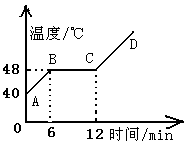
\includegraphics[width=\linewidth]{figures/图片1.png} 
\columnbreak
\begin{choices}
\choice 海波的沸点是48℃
\choice 海波在BC段吸收了热量
\choice 海波在CD段是气态
\choice 6min时海波已全部熔化
\end{choices}
\end{multicols}



\question
在透明塑料袋中滴入几滴酒精,将袋挤瘪,排尽袋中空气后 把口扎紧,然后放入80℃以上的热水中,过一会儿,塑料袋鼓起;从热水中拿出塑料袋,过一会儿(\answerline*[D])
\begin{choices}
\choice 塑料袋仍然鼓起,其中的酒精液化了
\choice 塑料袋仍然鼓起,其中的酒精汽化了
\choice 塑料袋又瘪了,其中的酒精汽化了
\choice 塑料袋又瘪了,其中的酒精液化了
\end{choices}  




\end{questions}


\begin{advanceexercises}
\section{提高题}

\end{advanceexercises}


%\section{小信息}
%\showendnotes

\ThisCenterWallPaper{1}{教案模板-3.pdf}

\end{document}



